\documentclass[pmlr]{jmlr}

\usepackage{booktabs}
\usepackage{amsmath}
\usepackage[letterpaper,margin=1in]{geometry}% CFP: 1in margins (overrides jmlr's 1.25in)

\jmlrvolume{}
\jmlryear{2026}
\jmlrworkshop{Machine Learning in Computational Biology (MLCB)}

\title[How Much of gLM Variant-Effect Prediction Is Base Composition?]{How Much of Genomic Language Model Variant-Effect Prediction Is Base Composition?}

\author{\Name{Rikhin Kavuru} \Email{rikhinkavuru@gmail.com}\\
 \addr Independent Author}

\begin{document}

\maketitle

\begin{abstract}
Zero-shot variant-effect prediction (VEP) with genomic language models (gLMs) scores a
variant by the log-likelihood ratio $\mathrm{LLR}=\log p(\text{alt})-\log p(\text{ref})$.
This quantity mixes learned regulatory function with a purely local signal, namely how
mutationally expected a substitution is given its base composition and sequence context.
We isolate and quantify this composition/mutation-expectedness axis as a confound on real
clinical and functional VEP benchmarks, across nine gLMs and four benchmark families, using
only context-free features that require no learning. A composition-only classifier reaches
AUROC $0.720$ on noncoding ClinVar and recovers $45$--$53\%$ of the above-chance AUROC of
every leading model, including Evo2-40B, GPN-MSA, CADD and phyloP; the result is unchanged
when coding-overlapping variants are removed. On carefully composition-matched benchmarks
(TraitGym) the same baseline recovers only $17$--$25\%$, so matching removes roughly half of
the confound but not all of it. The confound is strongly
model dependent: smaller single-sequence gLMs (Nucleotide Transformer, Caduceus, HyenaDNA)
do not exceed the composition baseline on any benchmark, while alignment-based
(GPN-MSA) and large autoregressive (Evo2-40B) models retain signal that survives
composition matching and concentrates on TF-motif-disrupting variants (odds ratio up to
$5.4$). Within saturation-mutagenesis screens with fixed background the leakage is
negligible, which localises the confound to across-set ascertainment rather than local
context. We provide a model-agnostic post-hoc pentanucleotide calibration that halves the
mutation-rate coupling of the most affected model at negligible AUROC cost, and release it
as a drop-in evaluation transform.
\end{abstract}

\begin{keywords}
genomic language models, variant effect prediction, benchmark confounds, base composition,
mutation rate, calibration
\end{keywords}

\section{Introduction}
\label{sec:intro}

Genomic language models are increasingly presented as general predictors of noncoding
variant effect. The headline evidence is zero-shot: a pretrained model scores a single
nucleotide variant (SNV) by the log-likelihood ratio between the alternate and reference
alleles, $\mathrm{LLR}=\log p(\text{alt})-\log p(\text{ref})$, and this score is ranked
against clinical or functional labels \citep{benegas2025gpnmsa,brixi2026evo2}. Reported
aggregate AUROCs on noncoding ClinVar routinely exceed $0.95$, which is often read as
evidence that the models have learned regulatory grammar.

Three recent results complicate that reading. On designed synthetic promoters, the
compositional sensitivity of gLMs tracks AT content almost perfectly and a small
position-aware model beats billion-parameter gLMs \citep{mit2026}. Stratifying ClinVar by
region type collapses Evo2's aggregate noncoding AUROC because pathogenic variants
concentrate in easy region categories \citep{lu2025heterogeneity}. Cyclic permutation of
flanking context collapses Evo2 tRNA sensitivity, which shows that predictions ride on
irrelevant genomic context \citep{mathur2026blindspots}. Separately,
\citet{tang2025koo} report that frozen gLM representations give little advantage over
one-hot encodings on cell-type-specific regulatory tasks, and information-theoretic analyses
find that the usable information in genomic foundation models concentrates in embedding
rather than transformer layers \citep{entropy2026}.

These studies identify positional-grammar, region-type and context-artifact confounds. We
study a distinct axis that none of them isolates on real VEP: local \emph{base composition}
and \emph{mutational expectedness}. The mechanism is direct. A model's likelihood partly
encodes how expected a substitution is under neutral evolution. CpG transitions mutate an
order of magnitude faster than transversions, the transition/transversion ratio is a
function of local CpG content, and mutation subtype couples to GC background
\citep{carlson2018mutrate}. Because pathogenic and causal variants are ascertained
non-randomly across mutation types, the mutation-expectedness component of LLR correlates
with labels for reasons unrelated to regulatory understanding. This is precisely why
CADD and GPN-MSA use common variants rather than ClinVar-benign as controls
\citep{rentzsch2019cadd,benegas2025gpnmsa}. \citet{gpnstar2025} reported that raw gLM scores
correlate with pentanucleotide mutation-rate estimates at $\rho=0.31$--$0.34$ and introduced
a per-context calibration for a single model as a training-adjacent step.

\paragraph{Contributions.} We turn that observation into a benchmark-wide, cross-model,
post-hoc audit. (1) We show a context-free composition baseline recovers about half of the
above-chance AUROC of every leading model on unmatched ClinVar, and about a fifth on
composition-matched TraitGym, which quantifies how much aggregate-leaderboard performance is
composition-attributable (\S\ref{sec:e2}). (2) We show the confound is model-heterogeneous:
smaller single-sequence gLMs are indistinguishable from the baseline, whereas alignment-based
and large autoregressive models keep signal that survives composition matching
(\S\ref{sec:e1}, \S\ref{sec:e3}). (3) We localise the confound to across-set ascertainment
rather than local context using within-element saturation mutagenesis (\S\ref{sec:e4}).
(4) We generalise pentanucleotide calibration into a model-agnostic post-hoc transform and
release it (\S\ref{sec:e5}). (5) We map where genuine gLM signal survives, namely
TF-motif-disrupting variants (\S\ref{sec:e6}). Our framing follows the confound-audit genre
of \citet{gupta2025background}: name a hidden confound, build a clean evaluation, measure its
effect across a model class, and localise where real signal remains.

\section{The composition and mutation-expectedness confound}
\label{sec:confound}

We define two entangled axes, both computed with no learning, for an SNV at position $p$
with reference and alternate alleles.

\paragraph{C1, local composition change.} For window half-width $w$, let $s_{\text{ref}}$ and
$s_{\text{alt}}$ be the $\pm w$ sequences. We take $\Delta_k$, the $L_1$ distance between the
$k$-mer frequency spectra of $s_{\text{ref}}$ and $s_{\text{alt}}$ for $k\in\{1,2,3\}$, and
$\Delta\mathrm{GC}=|\mathrm{GC}(s_{\text{alt}})-\mathrm{GC}(s_{\text{ref}})|$, sweeping
$w\in\{11,21,51\}$ bp.

\paragraph{C2, mutational expectedness.} The pentanucleotide neutral mutation rate for the
specific substitution \citep{carlson2018mutrate}, the CpG status of the reference and
alternate sites, the transition/transversion class, and the flanking GC background.

All features are strand-invariant by construction. Under a simple mechanism model
$\mathrm{LLR}\approx\alpha\cdot(\text{function})+\beta\cdot(\text{expectedness})+\varepsilon$,
the confound is the $\beta$ term. It correlates with labels through ascertainment, not
through regulatory understanding. Matching and calibration target $\beta$; the residual
$\alpha$ is what a gLM should contribute beyond a mutation-rate lookup.

\section{Experimental setup}
\label{sec:setup}

\paragraph{Benchmarks.} \emph{ClinVar noncoding} ($153{,}508$ SNVs, $25{,}571$ pathogenic):
$\geq$2-star pathogenic/likely-pathogenic versus benign/likely-benign SNVs overlapping an
ENCODE candidate cis-regulatory element (cCRE) \citep{encode2020ccre}; region-heterogeneous
and unmatched, so the confound should be largest. \emph{TraitGym} Mendelian ($3{,}380$;
$338$ positive) and complex ($11{,}400$; $1{,}140$) \citep{benegas2025traitgym}: fine-mapped
causal regulatory variants matched on chromosome, consequence, distance to transcription
start site (TSS), and for complex traits also minor allele frequency (MAF) and linkage
disequilibrium (LD), so the confound should be smallest. \emph{Kircher} saturation
massively-parallel reporter assay (MPRA) \citep{kircher2019satmut}: $39{,}170$ SNVs across
$21$ elements with a continuous log$_2$ expression effect and fixed within-element
background. \emph{Genomics Long-Range Benchmark (GLRB) causal expression QTL}
\citep{glrb2024}: $8{,}850$ held-out test SNVs where zero-shot DNA LMs are known to be near
chance.

\paragraph{Models.} We use authors' released per-variant scores wherever available so that
model quality is not confounded by our own inference. On TraitGym this gives nine gLMs
(GPN-MSA, an alignment-based multiple-sequence-alignment (MSA) model; Evo2-1B/7B/40B;
Nucleotide Transformer; Caduceus; HyenaDNA; SpeciesLM; and AIDO.DNA) plus CADD, phyloP and
phastCons. On ClinVar we use precomputed Evo2-7B/40B and Nucleotide Transformer scores
together with a genome-wide GPN-MSA tabix lookup, CADD, phyloP and SpliceAI. GPN-MSA is the
alignment-based anchor present on every benchmark. Our composition baseline is a
histogram gradient-boosted-tree classifier (250 trees, learning rate $0.05$) on the $19$
C1/C2 features only (the $\Delta_k$ and $\Delta$GC values at the three windows, the
pentanucleotide rate, CpG and transition indicators, and flanking GC), with no sequence
context and no embedding.

\paragraph{Protocol.} We report the area under the ROC curve (AUROC) and the area under the
precision-recall curve (AUPRC), oriented so that higher scores indicate the positive class.
Binary benchmarks use leave-one-chromosome-out cross-validation with sample-size-weighted
averaging \citep{benegas2025traitgym}. We use partial Spearman correlations controlling for
consequence or region, the paired DeLong test for AUROC differences, Benjamini--Hochberg
control across model$\times$benchmark comparisons, and percentile bootstrap intervals. The
composition classifier is trained under the same leave-one-chromosome-out folds as the
evaluation so that recovery ratios are comparable and no variant informs its own fold.

\section{Results}

\subsection{E1: gLM scores encode the confound, model-dependently}
\label{sec:e1}

Figure~\ref{fig:confound}(a) reports the partial Spearman correlation between $|\mathrm{LLR}|$
and the pentanucleotide mutation rate, controlling for consequence. GPN-MSA is the most
strongly coupled model at $\rho=-0.33$ on ClinVar and $-0.16$ to $-0.20$ on TraitGym,
consistent with an alignment model that tracks neutral rate. Evo2-40B is intermediate
($-0.08$ to $-0.18$), Evo2-7B is weak ($\approx-0.04$), and the smaller single-sequence
models (Nucleotide Transformer, Caduceus, HyenaDNA) are near zero. Conservation baselines
show similar coupling to the models. The confound is present but is not uniform across the
model class.

This coupling is not an artifact of the labelled sets. At genome-wide neutral sites, GPN-MSA's
mean score per pentanucleotide context tracks the Carlson neutral mutation rate at Spearman
$\rho=0.63$ ($p<10^{-16}$, all $3{,}072$ contexts, from $3.6\times10^{7}$ sampled scores):
highly mutable contexts, above all CpG sites, receive systematically less deleterious scores
(mean $-0.10$ at CpG-centred contexts versus $-1.33$ elsewhere). The model has learned the
neutral mutation spectrum, which is exactly the component that leaks into the LLR when
variants are ascertained non-randomly across mutation types.

That ascertainment is directly visible in the labels. In ClinVar, benign SNVs sit at higher
mutation-rate contexts than pathogenic ones (mean pentanucleotide rate $0.033$ versus $0.028$,
$p<10^{-140}$), are more often transitions ($76\%$ versus $65\%$, $p<10^{-290}$), and more
often CpG ($35\%$ versus $31\%$). A score that encodes the neutral spectrum therefore separates
the two classes without any regulatory understanding, which is the label pathway the confound
travels.

\begin{figure}[t]
\centering

\includegraphics[width=\linewidth]{figures/fig2_confound.pdf}
\caption{\textbf{Confound structure.} (a) Partial $|\rho|$ between $|\mathrm{LLR}|$ and the
5-mer mutation rate per model and benchmark. GPN-MSA is most coupled. (b) Collapse curve on
TraitGym Mendelian: model AUROC minus composition AUROC within $|\Delta\mathrm{GC}|$
quartiles. Smaller single-sequence gLMs (dashed) hold no edge over composition in any bin;
alignment-based and large models keep a stable edge.}
\label{fig:confound}
\end{figure}

\subsection{E2: a composition baseline recovers much of aggregate performance}
\label{sec:e2}

On ClinVar the composition-only classifier reaches AUROC $0.720$ (bootstrap 95\% confidence
interval, CI, $0.716$--$0.722$) with no sequence context and no model. The leading models reach $0.958$
(GPN-MSA), $0.960$ (Evo2-7B), $0.963$ (Evo2-40B), $0.986$ (CADD) and $0.912$ (phyloP), so the
recovery ratio $(\text{comp}-0.5)/(\text{model}-0.5)$ is $0.45$--$0.53$ for every one of them
(all DeLong $p\approx 0$; the baseline is below each model, but recovers roughly half of its
above-chance discrimination). On composition-matched TraitGym the same baseline reaches only
$0.586$ (Mendelian) and $0.520$ (complex), with recovery ratios of $0.21$--$0.25$ and
$0.17$--$0.25$ against the models that clear chance. On GLRB causal eQTL the baseline
($0.596$) matches or exceeds GPN-MSA ($0.560$), so the little signal present is
composition-explainable. Table~\ref{tab:main} reports the full comparison and
Figure~\ref{fig:recovery} summarises the roughly two-fold difference between unmatched and
matched benchmarks. The difference is significant: the composition-only AUROC is $0.720$
(bootstrap 95\% CI $0.716$--$0.722$) on ClinVar versus $0.586$ ($0.556$--$0.613$) on TraitGym
Mendelian and $0.520$ ($0.503$--$0.540$) on complex, with non-overlapping intervals, while the
model AUROC intervals are narrow given $n>10^4$. Matching removes about half of the confound,
which is a positive result for TraitGym, but a measurable residual leaks past even MAF- and
LD-matched controls.

The ClinVar result is not an artifact of coding overlap. Restricting to the strict-noncoding
subset that excludes the $46{,}852$ variants annotated as coding ($106{,}656$ SNVs remain)
leaves the composition baseline at AUROC $0.734$ and every recovery ratio in the
$0.48$--$0.50$ range, essentially unchanged from the full set.

The recovery ratio measures how much of the above-chance AUROC a trivial baseline reaches, not
a decomposition of the model, so we also test unique contribution by training composition and
model features together under the same folds. On ClinVar, adding GPN-MSA to the composition
features raises AUROC from $0.717$ to $0.971$ ($+0.254$), while adding composition to GPN-MSA
raises it by only $+0.013$; the pattern holds for Evo2-40B ($+0.193$ versus $+0.057$) and on
TraitGym Mendelian ($+0.306$ versus $+0.007$). The strong models thus subsume the composition
signal and carry large composition-independent signal on top of it, whereas the smaller
single-sequence gLMs do not exceed composition at all (Table~\ref{tab:main}). The confound
inflates the leaderboard \emph{impression}, since a context-free baseline already scores high,
without implying that the stronger models are reducible to composition.

\begin{figure}[t]
\centering
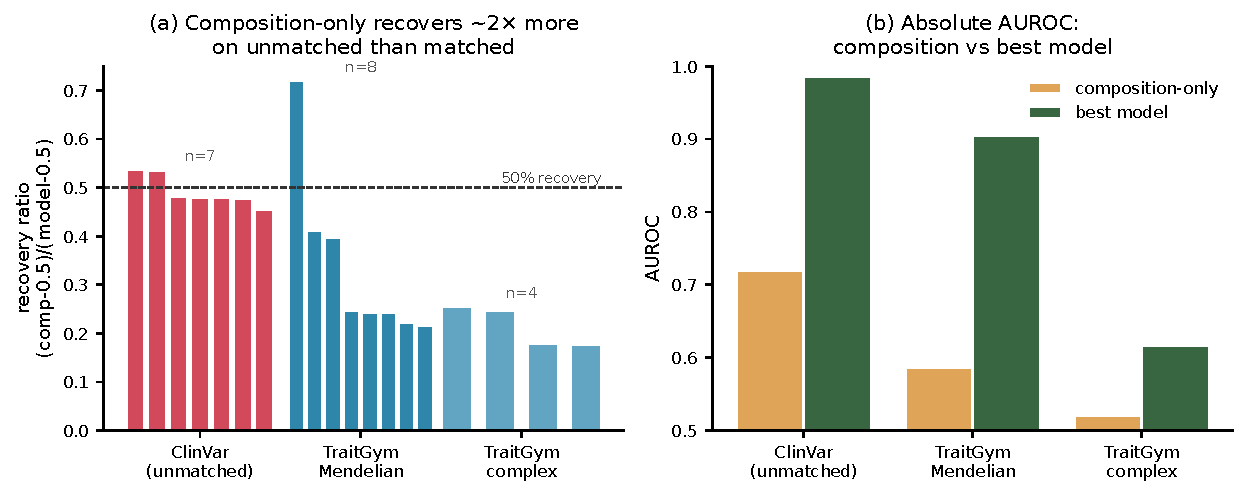
\includegraphics[width=\linewidth]{figures/fig1_recovery.pdf}
\caption{\textbf{Composition recovery.} (a) Recovery ratio per model, grouped by benchmark;
composition recovers about twice as much above-chance AUROC on unmatched ClinVar as on
matched TraitGym. (b) Absolute AUROC of the composition baseline versus the best model per
benchmark.}
\label{fig:recovery}
\end{figure}

\begin{table}[t]
\centering
\caption{Leave-one-chromosome-out AUROC with per-chromosome stratified-bootstrap 95\% CIs,
AUPRC, and the composition recovery ratio
$(\text{AUROC}_{\text{comp}}-0.5)/(\text{AUROC}_{\text{model}}-0.5)$ for the composition
baseline versus each model. A recovery ratio above one (marked $>$1) means the model does not
exceed the composition baseline. Composition and model AUROC CIs are non-overlapping on every
matched-vs-unmatched contrast, and all model-vs-composition DeLong tests give $p<10^{-3}$
except the near-chance single-sequence gLMs on complex traits ($p>0.7$).}
\label{tab:main}
\small
\begin{tabular}{lccc}
\toprule
Method & AUROC [95\% CI] & AUPRC & Recovery \\
\midrule
\multicolumn{4}{l}{\emph{ClinVar (unmatched)}}\\
\quad Composition-only & 0.720 [0.716,0.723] & 0.362 & -- \\
\quad GPN-MSA & 0.958 [0.957,0.960] & 0.861 & 0.48 \\
\quad Evo2-7B & 0.960 [0.959,0.962] & 0.882 & 0.48 \\
\quad Evo2-40B & 0.963 [0.962,0.965] & 0.870 & 0.47 \\
\quad CADD & 0.986 [0.985,0.987] & 0.958 & 0.45 \\
\quad phyloP & 0.912 [0.909,0.914] & 0.775 & 0.53 \\
\addlinespace
\multicolumn{4}{l}{\emph{TraitGym Mendelian (matched)}}\\
\quad Composition-only & 0.586 [0.559,0.617] & 0.153 & -- \\
\quad GPN-MSA & 0.904 [0.886,0.921] & 0.694 & 0.21 \\
\quad Evo2-7B & 0.710 [0.682,0.743] & 0.385 & 0.41 \\
\quad Evo2-40B & 0.851 [0.830,0.872] & 0.557 & 0.25 \\
\quad NT-2.5B & 0.534 [0.508,0.566] & 0.120 & $>$1 \\
\quad Caduceus & 0.509 [0.483,0.539] & 0.108 & $>$1 \\
\quad CADD & 0.893 [0.871,0.914] & 0.712 & 0.22 \\
\quad phyloP & 0.857 [0.830,0.883] & 0.655 & 0.24 \\
\addlinespace
\multicolumn{4}{l}{\emph{TraitGym complex (matched)}}\\
\quad Composition-only & 0.520 [0.499,0.537] & 0.115 & -- \\
\quad GPN-MSA & 0.580 [0.562,0.600] & 0.212 & 0.25 \\
\quad Evo2-40B & 0.516 [0.498,0.534] & 0.137 & 1.26 \\
\quad NT-2.5B & 0.516 [0.500,0.534] & 0.114 & $>$1 \\
\quad Caduceus & 0.518 [0.502,0.536] & 0.114 & $>$1 \\
\quad CADD & 0.616 [0.598,0.637] & 0.250 & 0.18 \\
\quad phyloP & 0.583 [0.565,0.604] & 0.184 & 0.24 \\
\addlinespace
\multicolumn{4}{l}{\emph{GLRB eQTL}}\\
\quad Composition-only & 0.596 [0.585,0.607] & 0.633 & -- \\
\quad GPN-MSA & 0.560 [0.548,0.571] & 0.599 & $>$1 \\
\bottomrule
\end{tabular}
\end{table}

\subsection{E3: matching shrinks but does not erase the gLM edge}
\label{sec:e3}

Figure~\ref{fig:confound}(b) bins TraitGym Mendelian variants by $|\Delta\mathrm{GC}|$ and
plots each model's AUROC minus the composition AUROC. Nucleotide Transformer, Caduceus and
HyenaDNA hold no edge in any bin, so their apparent VEP signal is composition. GPN-MSA,
Evo2-40B, CADD and phyloP keep a stable edge of roughly $0.24$. We then nearest-neighbour
match positives to controls on the C1/C2 features within consequence class, on top of
TraitGym's own matching. Model AUROC drops only slightly under this stricter matching
(ClinVar GPN-MSA $-0.006$, TraitGym Mendelian Evo2-40B $-0.019$, Nucleotide Transformer
$-0.025$), and the model ranking reorders mildly (Kendall $\tau=0.81$--$0.91$). The models
that clear chance therefore carry composition-independent signal.

\subsection{E4: within fixed background the leakage is negligible}
\label{sec:e4}

The Kircher screens fix the background sequence within each element, which isolates the
substitution and its immediate context. For each of the $21$ elements we regress GPN-MSA LLR
on the measured log$_2$ effect and compare the raw Spearman correlation with a partial
correlation controlling for substitution type, $\Delta\mathrm{GC}$ and CpG status. The
partial and raw correlations nearly coincide (mean absolute change below $0.02$;
Figure~\ref{fig:within}(a)), so within a fixed background the model--assay correlation is not
a composition artifact. Combined with E2, this localises the confound to across-set
ascertainment rather than to local context.

\begin{figure}[t]
\centering
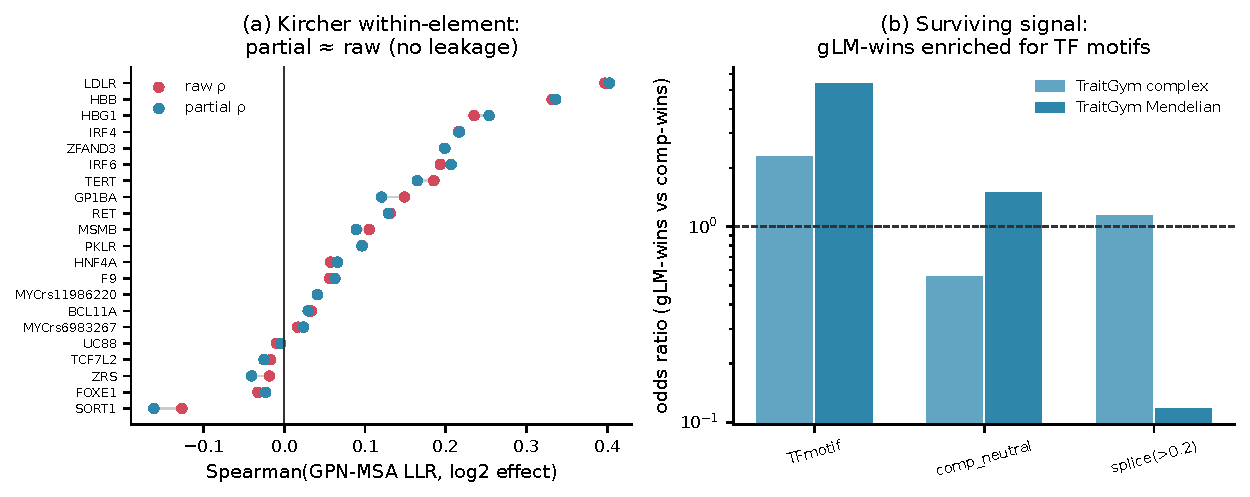
\includegraphics[width=\linewidth]{figures/fig4_within_surviving.pdf}
\caption{\textbf{Localisation and surviving signal.} (a) Kircher within-element raw versus
partial Spearman of GPN-MSA LLR against measured effect; the two nearly coincide.
(b) Odds ratios for gLM-wins versus composition-wins among positives; gLM-wins are enriched
for TF-motif and footprint overlap.}
\label{fig:within}
\end{figure}

\subsection{E5: a model-agnostic pentanucleotide calibration}
\label{sec:e5}

We define a post-hoc transform that subtracts a per-pentanucleotide-context neutral score,
estimated leave-one-chromosome-out from control variants only, so that no test-fold label is
used. On ClinVar this halves the mutation-rate coupling of GPN-MSA (partial $\rho$ from
$-0.33$ to $-0.17$) and reduces Evo2-40B coupling, at an AUROC cost below $0.005$
(Figure~\ref{fig:calib}). The leaderboard reorders mildly (Kendall $\tau=0.80$ on ClinVar,
$0.91$ on TraitGym). A label-free alternative estimator, a genome-wide neutral table built
from $3{,}072$ pentanucleotide contexts and $3.6\times10^{7}$ sampled genome-wide GPN-MSA
scores in the manner of \citet{gpnstar2025}, reproduces the effect and is if anything cleaner:
it reduces GPN-MSA's mutation-rate coupling from $0.33$ to $0.18$ while leaving AUROC
unchanged ($0.958$ to $0.961$). The small AUROC effect is consistent with E3 and E4:
calibration is a decontamination diagnostic that removes the mutation-rate coupling without
destroying the signal the stronger models genuinely carry. We release the transform as a
drop-in \texttt{calibrate\_llr} function together with the per-context neutral tables.

\begin{figure}[t]
\centering

\includegraphics[width=\linewidth]{figures/fig3_calibration.pdf}
\caption{\textbf{Post-hoc calibration.} (a) Mutation-rate coupling before and after
calibration on ClinVar; the most coupled model (GPN-MSA) is halved. (b) AUROC before versus
after calibration; points lie near the diagonal, so the decontamination cost is small.}
\label{fig:calib}
\end{figure}

\subsection{E6: surviving signal is motif-disrupting}
\label{sec:e6}

Among positives, we compare variants that the calibrated GPN-MSA ranks highly but the
composition baseline misses (``gLM-wins'') against the reverse (``composition-wins'').
gLM-wins are enriched for overlap with transcription-factor (TF) motifs and ChIP footprints,
with odds ratio $5.4$ on TraitGym Mendelian and $2.3$ on complex (Figure~\ref{fig:within}(b));
the Mendelian estimate rests on a small composition-win set and should be read as
directional. Splice-proximity and
composition-neutral enrichments are weaker and noisier, as expected given how few splice
variants fall in the noncoding-regulatory set. The signal that survives decontamination
concentrates on regulatory grammar, namely motif disruption, which is where the gLM claim is
genuinely testable.

\section{Discussion}
\label{sec:discussion}

Our results support a specific and calibrated claim rather than a blanket dismissal. A
context-free composition and mutation-rate baseline recovers about half of the apparent
zero-shot VEP performance of leading gLMs on the unmatched, region-heterogeneous benchmarks
that dominate reported leaderboards, and about a fifth on carefully matched benchmarks. The
confound bites hardest on the smaller single-sequence gLMs, which do not exceed the
baseline on any benchmark and sit at chance once benchmarks are matched. This is
consistent with \citet{tang2025koo}, who find that frozen gLM representations rarely beat
one-hot encodings. Alignment-based and large autoregressive models keep signal that survives
composition matching and concentrates on motif-disrupting variants. The confound is an
across-set ascertainment phenomenon and not a local-context artifact, since it vanishes
within fixed-background saturation screens.

\paragraph{Limitations.} We score zero-shot LLR, which is the deployed clinical setting and
the headline claim in gLM VEP papers, but not the only use of these models; fine-tuning is
out of scope and we include CADD and conservation to bound the integrative-model comparison.
Our composition features are a specific, if broad, operationalisation of the confound, and
the recovery ratio depends on classifier capacity, which we fix in advance. The ClinVar
noncoding set includes cCRE variants that also overlap coding annotations; a strict noncoding
subset is a natural robustness check. Composition and function are genuinely correlated, so
the goal is not to declare composition non-biological but to test whether a model advertised
as understanding regulatory grammar is reducible to a mutation-rate detector on the
benchmarks used to certify it.

\paragraph{Recommendations.} Report a composition baseline alongside gLM VEP, prefer matched
benchmarks or the calibrated score for cross-model comparison, and evaluate on
motif-disrupting variants where the grammar claim is testable.

\paragraph{Reproducibility.} All model scores are authors' released per-variant values
(TraitGym on the Hugging Face Hub, the goodarzilab Evo2-ClinVar release, and the songlab
genome-wide GPN-MSA scores) or public annotations (CADD, phyloP, phastCons, SpliceAI,
ENCODE cCREs). Composition features use the Carlson pentanucleotide mutation-rate table and
hg38. The feature, scoring, calibration, and evaluation code, the per-context neutral
tables, and the released \texttt{calibrate\_llr} transform are available at
\url{https://github.com/rikhinkavuru/composition-confound-vep}.

% Acknowledgements omitted for brevity.

\bibliography{references}

\end{document}
